\documentclass[10pt]{article}
\usepackage{latexsym}
\usepackage{natbib}
\usepackage{graphicx}
\usepackage{subfigure}
\usepackage{listings}
\usepackage{algorithm}
\usepackage{algpseudocode}

\title{Homework 1: Eigendigits}
\author{Shun Zhang}
\date{}

\begin{document}
\maketitle

\section{Introduction}

In this report, I apply principal components analysis on digits
classification problem. 60000 training samples and 10000 testing
samples are provided.

\section{Experiments}

On different size of data.

%hw1Classify(n, 1000, 200, 1)
\begin{figure}[b]
\centering
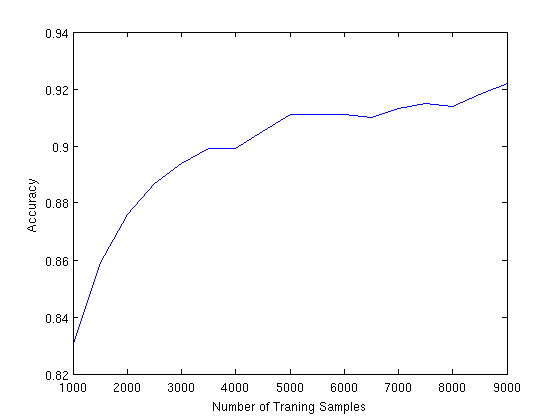
\includegraphics[width=0.8\columnwidth]{diffDataSet.png}
\caption{Comparison on using different number of training samples.
Testing on first 1000 testing set. Using first 200 eigen-vectors. K
for K-nearest-neighbors is 1.}
\label{fig:dataset}
\end{figure}

Using different number of eigenvectors.

\begin{figure}[b]
\centering
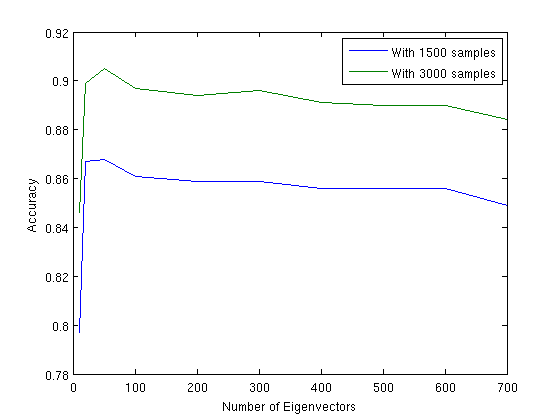
\includegraphics[width=0.8\columnwidth]{diffEVector.png}
\caption{Comparison on using different number of eigenvectors.
Testing on first 1000 testing set. Using first 1500 and 3000 training
samples for each line.  K for K-nearest-neighbors is 1.}
\label{fig:evec}
\end{figure}

\end{document}
